\documentclass[handout]{beamer}
%==============================================================
% Common Beamer Preamble for Course Lectures: Training and Scaling Language Models
%==============================================================

\usepackage[utf8]{inputenc}
\usepackage[T1]{fontenc}
\usepackage{hyperref}
\usepackage{amsmath,amssymb,xcolor,multicol,booktabs,colortbl}
\usepackage{graphicx,listings}
\renewcommand{\figurename}{Figure.}
\renewcommand{\tablename}{Table.}

% ---- TikZ Libraries ----
\usepackage{tikz}
\usetikzlibrary{positioning,arrows.meta,shapes.geometric,calc,fit,backgrounds,decorations.pathreplacing}

% ---- Presentation defaults ----
\setbeamertemplate{navigation symbols}{}
\setbeamersize{text margin left=0.55cm,text margin right=0.55cm}
\setbeamerfont{title}{size=\LARGE,series=\bfseries}
\setbeamerfont{subtitle}{size=\large}

% ---- FontAwesome fallback ----
\IfFileExists{fontawesome5.sty}{%
  \usepackage{fontawesome5}%
}{%
  \providecommand{\faMicrochip}{}%
  \providecommand{\faComments}{}%
  \providecommand{\faTools}{}%
  \providecommand{\faCheckCircle}{}%
  \providecommand{\faExclamationTriangle}{}%
  \providecommand{\faImage}{}%
  \providecommand{\faRobot}{}%
  \providecommand{\faTerminal}{}%
  \providecommand{\faBook}{}%
  \providecommand{\faRedo}{}%
  \providecommand{\faLayerGroup}{}%
  \providecommand{\faCogs}{}%
  \providecommand{\faDatabase}{}%
  \providecommand{\faHdd}{}%
  \providecommand{\faNetworkWired}{}%
}

% ---- Theme Style and Semantic Colors ----
%==============================================================
% Centralized Semantic Color Definitions for LLMs Presentation
%==============================================================

% ---- Base Template / Theme Colors (Aligned with Palette B) ----
\definecolor{themenavy}{RGB}{22,70,102}       % Palette B primary cerulean: #164666
\definecolor{themeblue}{RGB}{22,70,102}       % Primary alias
\definecolor{primarylight}{RGB}{34,92,132}    % Primary light: #225c84
\definecolor{themeteal}{RGB}{0,159,176}       % Accent cyan-teal: #009fb0
\colorlet{main_color}{themenavy}
\colorlet{accent}{themeteal}

\definecolor{accentdark}{RGB}{0,108,120}      % Deep cyan-teal for contrast text
\definecolor{accentlight}{RGB}{56,178,214}    % Slate accent cyan: #38b2d6
\definecolor{leafred}{RGB}{197,93,61}         % Terracotta red for branches/leaves

% ---- Website Panel & Border Neutrals ----
\definecolor{panelbg}{RGB}{237,245,249}       % Course-panel: #edf5f9
\definecolor{panelborder}{RGB}{204,226,238}   % Course-border: #cce2ee

% ---- Code listing style (syntax highlights) ----
\definecolor{deepblue}{RGB}{22,70,102}
\definecolor{deepred}{rgb}{0.6,0,0}
\definecolor{deepgreen}{RGB}{0,135,150}
\definecolor{halfgray}{gray}{0.55}

% ---- Semantic Theme Navy / Cerulean Shades ----
\colorlet{themebluebg}{panelbg}               % Panel #edf5f9
\colorlet{themebluecard}{main_color!8}        % Mild card background fills
\colorlet{themeblueborder}{panelborder}       % Border #cce2ee
\colorlet{themebluemid}{themeteal!60}         % Accent mid-contrast
\colorlet{themebluedraw}{main_color!80}       % Strong outline draws/strokes

% ---- Semantic Secondary Accent Teal Shades ----
\colorlet{accentdarkbg}{themeteal!10}        % Light secondary background fills
\colorlet{accentdarkdraw}{themeteal}         % Secondary outlines/strokes/text/axes

% ---- Functional Colors: Success Green ----
\definecolor{successgreen}{RGB}{55,145,55}
\colorlet{successbg}{successgreen!8}
\colorlet{successdraw}{successgreen!75}

% ---- Functional Colors: Alert Red ----
\definecolor{alertred}{RGB}{197,55,55}
\colorlet{alertbg}{alertred!8}
\colorlet{alertdraw}{alertred!75}

% ---- Functional Colors: Warning Orange ----
\definecolor{warningorange}{RGB}{220,110,30}
\colorlet{warningbg}{warningorange!10}
\colorlet{warningdraw}{warningorange!80}

% ---- Terracotta Red Shades ----
\colorlet{leafredbg}{leafred!12}
\colorlet{leafreddraw}{leafred!80}

% ---- Accent Violet (SWE-bench / observe phases) ----
\definecolor{accentviolet}{RGB}{120,70,180}
\colorlet{accentvioletbg}{accentviolet!10}
\colorlet{accentvioletdraw}{accentviolet!80}

% ---- Post-Training Axis Blue ----
\definecolor{posttrainingblue}{RGB}{40,90,165}
\colorlet{posttrainingbg}{posttrainingblue!8}
\colorlet{posttrainingdraw}{posttrainingblue!75}

% ---- Harness Component Action Green ----
\definecolor{actiongreen}{RGB}{55,145,55}
\colorlet{actiongreenbg}{actiongreen!10}
\colorlet{actiongreendraw}{actiongreen!65}

% ---- Harness Component Persist Olive ----
\definecolor{persistolive}{RGB}{120,135,40}
\colorlet{persistolivebg}{persistolive!12}
\colorlet{persistolivedraw}{persistolive!70}

% ---- Harness Component Observe Violet ----
\colorlet{observevioletbg}{accentvioletbg}
\colorlet{observevioletdraw}{accentvioletdraw}

% ---- Neutrals (Grays/Blacks) ----
\colorlet{neutralbg}{black!4}             % Very light background fills
\colorlet{neutrallight}{black!30}         % Border frames/ticks/dividers
\colorlet{neutraldark}{black!75}          % Main body text/code listing text

% ---- Beamer Block Color Overrides (Premium Terracotta Theme) ----
\setbeamercolor{block title alert}{bg=leafreddraw,fg=white}
\setbeamercolor{block body alert}{bg=leafredbg}
\setbeamercolor{alerted text}{fg=leafreddraw}

\usepackage{../common/style}
\graphicspath{{../common/figs/}{figs/}}

% ---- Code Listing Config ----
\lstset{
  basicstyle=\ttfamily\footnotesize,
  keywordstyle=\bfseries\color{deepblue},
  emphstyle=\ttfamily\color{deepred},
  stringstyle=\color{deepgreen},
  commentstyle=\color{halfgray}\itshape,
  numbers=left, numberstyle=\tiny\color{halfgray},
  backgroundcolor=\color{codebg},
  frame=l, framerule=1.5pt, rulecolor=\color{themeteal},
  xleftmargin=10pt, framexleftmargin=4pt, numbersep=6pt,
  showstringspaces=false, breaklines=true,
  aboveskip=4pt, belowskip=4pt
}

% ---- Image Placeholder Utility ----
\newcommand{\slideimage}[2][3.8cm]{%
  \begin{center}
    \begin{tikzpicture}
      \node[draw=main_color, dashed, very thick, rounded corners,
        fill=themebluebg, minimum width=0.88\linewidth, minimum height=#1,
      text width=0.80\linewidth, align=center, font=\itshape, text=accentdark]
      {\textbf{[ FIGURE / DIAGRAM ]}\\[6pt] #2};
    \end{tikzpicture}
  \end{center}
}

% ---- Concept Highlight Card Utility ----
\newcommand{\conceptcard}[3]{%
  \begin{coursebox}{#1}{#2}#3\end{coursebox}%
}

% ---- Reusable teaching-slide components ----
\newcommand{\learninggoals}[4]{%
  \begin{frame}{What should be clear by the end?}
    \begin{enumerate}
        \setlength{\itemsep}{7pt}
      \item #1
      \item #2
      \item #3
      \item #4
    \end{enumerate}
  \end{frame}
}

\newcommand{\checkpoint}[2]{%
  \begin{frame}{Checkpoint: #1}
    \begin{block}{Think, then compare}
      #2
    \end{block}
  \end{frame}
}

\newcommand{\takeaways}[4]{%
  \begin{frame}{The durable ideas}
    \begin{enumerate}
        \setlength{\itemsep}{8pt}
      \item #1
      \item #2
      \item #3
      \item #4
    \end{enumerate}
  \end{frame}
}

\newcommand{\smallsource}[1]{%
  \vfill\hfill{\tiny\color{neutraldark}Source: #1}
}

% ---- Logo on content frames ----
\newif\ifplacelogo
\placelogotrue
\logo{\ifplacelogo
  \raisebox{-0.3ex}{
\includegraphics[height=0.4cm]{IMT_Atlantique_logo.png}}%
\fi}

\makeatletter
\define@key{beamerframe}{nologo}[true]{%
  \placelogofalse
}
\makeatother

% Fix Beamer bold font warning: substitute undefined T1/cmss/b/n with T1/cmss/bx/n
\DeclareFontShape{T1}{cmss}{b}{n}{<->ssub * cmss/bx/n}{}

% Default Author & Institute metadata
\author[Jonathan Lys]{Jonathan Lys}
\institute[IMT Atlantique]{IMT Atlantique}

% ---- Front Page / Title Slide Macro ----
% Displays Title + IMT Atlantique logo and Brain logo
\newcommand{\makelecturetitle}[1][Training and Scaling Language Models: From First Principles to Efficient Serving]{%
  \placelogofalse
  {
    \setbeamertemplate{footline}{}
    \settitletagline{#1}
    \settitlelogos{%
      \raisebox{-0.5\height}{
\includegraphics[height=1.15cm]{IMT_Atlantique_logo.png}}%
      \hspace{1.2em}%
      \raisebox{-0.5\height}{\includegraphics[height=1.15cm]{brain.pdf}}}
    \begin{frame}[plain]
      \titlepage
    \end{frame}
  }
  \placelogotrue
}

% Section TOC Frame
\AtBeginSection[]{\coursesectiondivider}


\title[TLM -- Welcome]{Welcome to Training \& Scaling Language Models\\[4pt]
\normalsize\itshape Course Presentation: What We Will Do, Organization, and Projects}
\date{\today}

\begin{document}
\makelecturetitle[Training and Scaling Language Models: From First Principles to Efficient Serving]

\begin{frame}{What will you build in this course?}
  \begin{columns}[c]
    \begin{column}{0.54\linewidth}
      \textbf{Not an API-calling tutorial.}\\
      We open the engine from first principles:
      \begin{itemize}
        \setlength{\itemsep}{7pt}
        \item Start with raw, noisy web text.
        \item Build a decoder-only Transformer from scratch.
        \item Train, profile, and push a single GPU to its limits.
        \item Scale across multiple GPUs and nodes.
        \item Serve the trained model with low latency.
      \end{itemize}
    \end{column}
    \begin{column}{0.44\linewidth}
      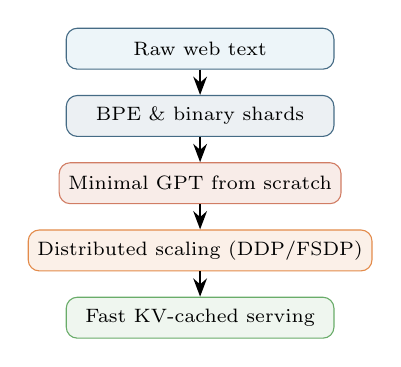
\begin{tikzpicture}[node distance=0.32cm, every node/.style={font=\scriptsize}]
        \node[draw=themebluedraw,fill=themebluebg,rounded corners,minimum width=3.4cm,minimum height=.52cm] (txt) {Raw web text};
        \node[draw=themebluedraw,fill=themebluecard,rounded corners,below=of txt,minimum width=3.4cm,minimum height=.52cm] (tok) {BPE \& binary shards};
        \node[draw=leafreddraw,fill=leafredbg,rounded corners,below=of tok,minimum width=3.4cm,minimum height=.52cm] (gpt) {Minimal GPT from scratch};
        \node[draw=warningdraw,fill=warningbg,rounded corners,below=of gpt,minimum width=3.4cm,minimum height=.52cm] (dist) {Distributed scaling (DDP/FSDP)};
        \node[draw=successdraw,fill=successbg,rounded corners,below=of dist,minimum width=3.4cm,minimum height=.52cm] (serve) {Fast KV-cached serving};
        \draw[-{Stealth},thick] (txt)--(tok);
        \draw[-{Stealth},thick] (tok)--(gpt);
        \draw[-{Stealth},thick] (gpt)--(dist);
        \draw[-{Stealth},thick] (dist)--(serve);
      \end{tikzpicture}
    \end{column}
  \end{columns}
\end{frame}

\begin{frame}{The governing question}
  Language models are limited by hardware physics, not just algorithms:
  \begin{columns}[t]
    \begin{column}{0.31\linewidth}
      \begin{block}{1. Compute wall}
        \small
        Tensor Cores require high arithmetic intensity:
        \vspace{2pt}
        \centering\small $\frac{\text{FLOPs}}{\text{Bytes transferred}}$
        \vspace{2pt}
        \raggedright Low intensity starves execution units.
      \end{block}
    \end{column}
    \begin{column}{0.31\linewidth}
      \begin{block}{2. Memory wall}
        \small
        Weights, optimizer states, activations, and KV cache compete for device RAM.
      \end{block}
    \end{column}
    \begin{column}{0.31\linewidth}
      \begin{block}{3. Network wall}
        \small
        NVLink and InfiniBand bandwidth limits distributed collective speed.
      \end{block}
    \end{column}
  \end{columns}
  \vspace{4pt}
  \begin{alertblock}{The question we answer in every module}
    Where is our system bottlenecked, and how do we prove an optimization actually works?
  \end{alertblock}
\end{frame}

\begin{frame}{The 3 phases of the course}
  \textbf{40 contact hours} organized into 32 sessions of 1h15:
  \begin{columns}[t]
    \begin{column}{0.32\linewidth}
      \begin{block}{Phase 1: Build (15h)}
        \footnotesize
        \textbf{Single-GPU foundation}
        \begin{itemize}
          \setlength{\itemsep}{1pt}
          \item Transformer architecture
          \item Training loop \& autograd
          \item Data pipeline \& BPE
          \item Profiling, MFU, FlashAttn
        \end{itemize}
      \end{block}
    \end{column}
    \begin{column}{0.32\linewidth}
      \begin{block}{Phase 2: Scale (15h)}
        \footnotesize
        \textbf{Distributed systems}
        \begin{itemize}
          \setlength{\itemsep}{1pt}
          \item Mid-course paper talks
          \item DDP (all-reduce)
          \item FSDP \& ZeRO sharding
          \item Tensor \& 5D parallelism
        \end{itemize}
      \end{block}
    \end{column}
    \begin{column}{0.32\linewidth}
      \begin{block}{Phase 3: Serve (10h)}
        \footnotesize
        \textbf{Inference \& synthesis}
        \begin{itemize}
          \setlength{\itemsep}{1pt}
          \item KV-cache decode
          \item Continuous batching
          \item Frontier architectures
          \item Final project defense
        \end{itemize}
      \end{block}
    \end{column}
  \end{columns}
  \vspace{3pt}
  \centering\small Each topic connects theory directly to measurable code.
\end{frame}

\begin{frame}{How sessions work: theory + hands-on practice}
  \begin{columns}[c]
    \begin{column}{0.52\linewidth}
      \conceptcard{themenavy}{Theory \& derivations}{%
        We unpack the mechanics: tensor shapes, autograd graphs, collective communication costs, and roofline models.
      }
      \vspace{6pt}
      \conceptcard{themeteal}{Guided implementation}{%
        You immediately build, test, and profile the mechanism using our companion PyTorch repository.
      }
    \end{column}
    \begin{column}{0.46\linewidth}
      \begin{block}{No waiting on progress bars}
        \begin{itemize}
          \setlength{\itemsep}{6pt}
          \item Class time is for \textbf{building, diagnosing, and measuring}.
          \item Long-running training jobs run asynchronously on the GPU cluster between sessions.
          \item Next class begins by analyzing the checkpoints, curves, and profiler traces.
        \end{itemize}
      \end{block}
    \end{column}
  \end{columns}
\end{frame}

\begin{frame}{The two projects}
  \begin{columns}[t]
    \begin{column}{0.48\linewidth}
      \begin{block}{1. The Continuous Laboratory}
        \textbf{The shared codebase everyone builds}
        \begin{itemize}
          \setlength{\itemsep}{5pt}
          \item In-class hands-on backbone.
          \item Every team builds the same evolving system from module 1 to 11.
          \item Validated by unit tests, shape checks, and profiler reports.
          \item Your sandbox and toolkit.
        \end{itemize}
      \end{block}
    \end{column}
    \begin{column}{0.48\linewidth}
      \begin{block}{2. The Reproduction Project}
        \textbf{The graded team challenge (65\%)}
        \begin{itemize}
          \setlength{\itemsep}{5pt}
          \item Pick a recent top-tier research paper (systems, scaling, data, efficiency).
          \item Scale down and verify \textbf{one precise claim} with controlled evidence.
          \item Supported by 4 dedicated in-class studio hackathons with instructors.
        \end{itemize}
      \end{block}
    \end{column}
  \end{columns}
\end{frame}

\begin{frame}{Reproduction project: what we expect}
  \begin{columns}[c]
    \begin{column}{0.51\linewidth}
      \begin{alertblock}{What NOT to do}
        Do not try to retrain a 70B model or reproduce an entire 20-page paper.
      \end{alertblock}
      \vspace{4pt}
      \begin{block}{Valid reproduction approaches}
        \begin{itemize}
          \setlength{\itemsep}{4pt}
          \item Test a memory or throughput claim under synthetic workloads.
          \item Test an architectural tweak on a smaller model (e.g.~124M).
          \item Verify a scaling law or ablation trend under a fixed compute budget.
        \end{itemize}
      \end{block}
    \end{column}
    \begin{column}{0.47\linewidth}
      \conceptcard{leafred}{Negative results welcome}{%
        A rigorous experiment that explains \emph{why} a published claim did not hold under controlled settings gets full credit.
      }
      \vspace{6pt}
      \conceptcard{successgreen}{Scientific rigor}{%
        Controlled variables, verified baselines, and clear ablations matter far more than raw model size.
      }
    \end{column}
  \end{columns}
\end{frame}

\begin{frame}{Grading and assessment}
  We grade engineering rigor, correct implementations, and controlled reasoning:
  \vfill
  \centering\small
  \begin{tabular}{lrp{5.2cm}}
    \toprule
    Component & Weight & Format \\
    \midrule
    \textbf{Pre-session quizzes} & \textbf{15\%} & 5-min online checks before each teaching day; verifies reading \& core concepts \\
    \addlinespace[4pt]
    \textbf{Mid-course paper talk} & \textbf{20\%} & 8-min presentation + 4-min Q\&A; explain the paper's mechanism \& proposed test \\
    \addlinespace[4pt]
    \textbf{Reproduction project} & \textbf{65\%} & Reproducible code, short technical report ($\le 5$ pages), and team defense with individual Q\&A \\
    \bottomrule
  \end{tabular}
  \vfill
  \raggedright\scriptsize Quizzes drop the lowest scores to accommodate occasional technical issues or absences.
\end{frame}

\begin{frame}{Course toolkit and logistics}
  \begin{columns}[c]
    \begin{column}{0.54\linewidth}
      \begin{itemize}
        \setlength{\itemsep}{6pt}
        \item \textbf{Companion repo}: \texttt{llm-course-companion}
        \item Clean, modular PyTorch implementation for each module.
        \item Automated test suites:
          \begin{itemize}
            \item Tensor shape invariants
            \item Causal masking checks
            \item Tiny-batch overfit ($L < 0.1$)
            \item Checkpoint resume determinism
          \end{itemize}
        \item Fast dependency management with \texttt{uv}.
        \item Dedicated GPU compute nodes for training runs.
      \end{itemize}
    \end{column}
    \begin{column}{0.44\linewidth}
      \begin{block}{Sanity check before Session 1}
        \ttfamily\scriptsize
        \# Clone \& install\\
        git clone <repo-url>\\
        cd llm-course-companion\\
        uv sync\\
        \vspace{4pt}
        \# Check GPU \& tests\\
        nvidia-smi\\
        uv run pytest tests/
      \end{block}
    \end{column}
  \end{columns}
\end{frame}

\begin{frame}{Summary: our contract}
  \begin{enumerate}
    \setlength{\itemsep}{9pt}
    \item \textbf{First principles}: No black boxes. We understand every tensor shape, CUDA kernel launch, and collective communication.
    \item \textbf{Measure before optimizing}: Trust profiler traces and MFU, not intuition.
    \item \textbf{Build together, explore in teams}: Master the fundamentals in the continuous lab, then test cutting-edge research in your reproduction project.
    \item \textbf{Rigorous science}: Real engineering is about reproducible baselines and honest analysis of trade-offs.
  \end{enumerate}
  \vfill
  \centering\large\color{themenavy}\textbf{Let's build a language model!}
\end{frame}

\end{document}
